\section{Seguimiento}
\subsection{Beneficio del framework Scrum}
El seguimiento del proyecto, utilizando la asignaci\'on de tareas por intermedio de RallyDev no nos result\'o beneficiosa. As\'i como en otros escenarios (laborales por ejemplo) donde el seguimiento de las horas es informado a un stakeholder con inter\'es en el avance, no nos dio resultados para mantener la velocidad esperada. Esto se refleja en el burndownchart donde se observa una s\'ubita ca\'ida en las horas faltantes para finalizar el sprint.

Los motivos para esto son diversos:
\begin{itemize}
    \item Conocimiento grupal de las tareas 
    \item Y de lo faltante (mucha comunicaci\'on por mail)
    \item Falta de comunicaci\'on del equipo con el stakeholder (falta de presi\'on acaso?)
\end{itemize}

Cabe mencionar que al no poder realizar actualización de horas retroactivas, algo bastante común de realizar en otras herramientas de seguimiento, el burnout chart no es fiel reflejo de nuestro avance.

La utilizaci\'on de Scrum para el manejo del proyecto nos brindó muchos beneficios en la primer etapa de an\'alis siendo una heramienta de mucha ayuda al descomponer los requerimientos en user stories y luego en tareas.

\subsection{Burndown chart}
\begin{figure}[ht]
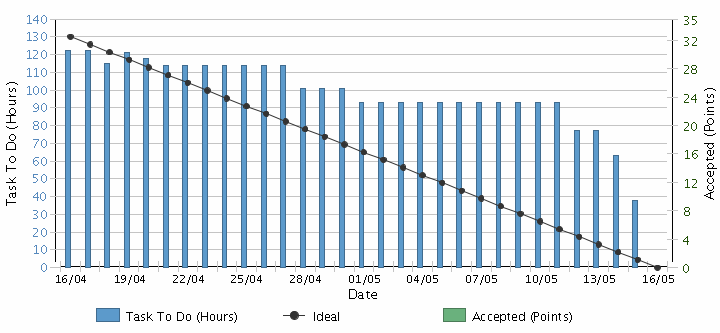
\includegraphics[width=\textwidth]{./imgs/burndown.png}
\end{figure}
